\begin{figure}
  \centering
  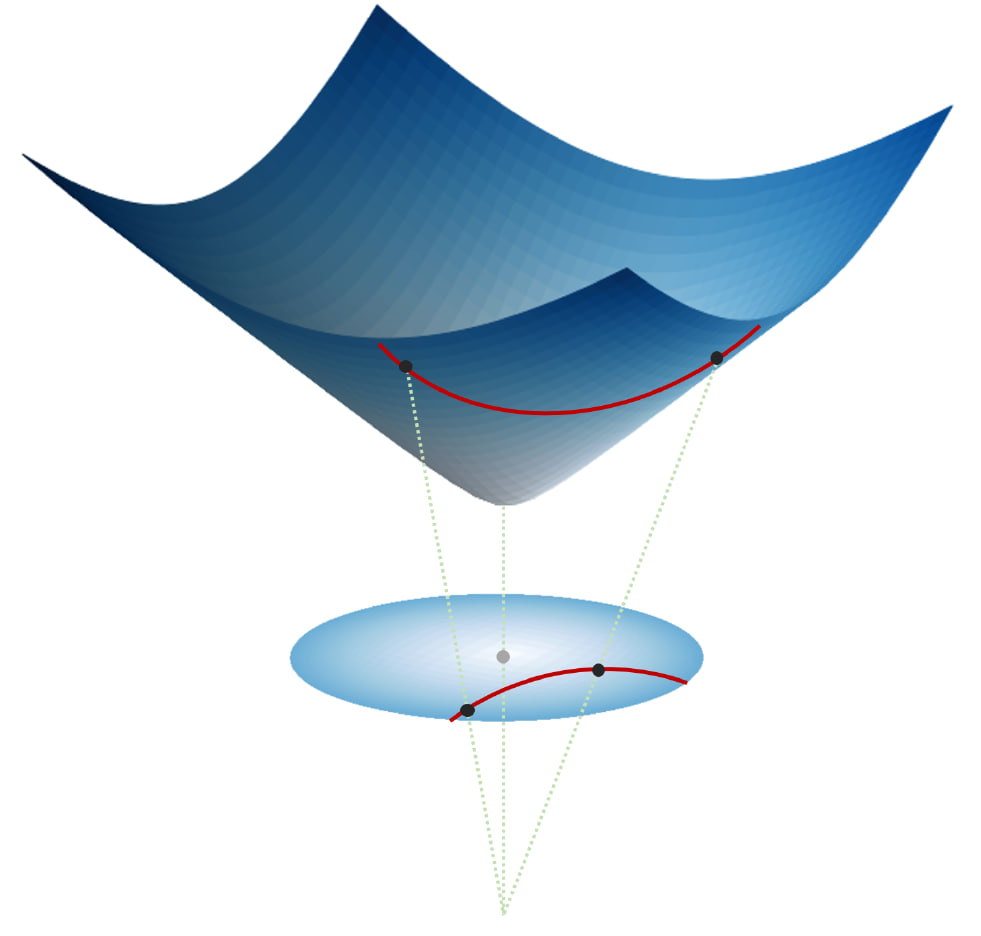
\includegraphics[width=0.5\textwidth]{figs/hyperboloidToPoincare.jpg}

    % \begin{tikzpicture}
    %   \begin{axis}[
    %     view={30}{10},
    %     colormap name=custom,
    %     shader=interp,
    %     axis lines=none,
    %     xmin=-3, xmax=3,
    %     ymin=-3, ymax=3,
    %     zmin=0, zmax=5,
    % ]
    
    % % Upper sheet of hyperboloid
    % \addplot3[
    %     surf,
    %     domain=-2.8:2.8,
    %     y domain=-2.8:2.8,
    %     samples=20,
    %     z buffer=sort,
    %     opacity=0.7
    % ] {sqrt(x^2 + y^2 + 1)};
    
    % % Geodesic curve (properly bounded)
    % \addplot3[
    %     red,
    %     thick,
    %     samples=20,
    %     samples y=0,
    %     domain=-1.8:2\,  % Match the hyperboloid's x-domain
    % ] (
    %     {x},
    %     {1},
    %     {sqrt(x^2 + 2)}  % Changed from +4 to +1 to stay on the surface
    % );
    
    % \end{axis}
    % \end{tikzpicture}
  \caption{Illustration of the hyperboloid (top) and its connection to the Poincaré ball (bottom)\cite{Chami2021representationLearningAlgorithmsHyperbolicSpaces}.}
  \label{fig:hyperboloidToPoincareBall}
\end{figure}